\documentclass[10pt,landscape,a4paper]{article}
\usepackage[utf8]{inputenc}
\usepackage[ngerman]{babel}
\usepackage{tikz}
\usetikzlibrary{shapes,positioning,arrows,fit,calc,graphs,graphs.standard}
\usepackage[nosf]{kpfonts}
\usepackage[t1]{sourcesanspro}
%\usepackage[lf]{MyriadPro}
%\usepackage[lf,minionint]{MinionPro}
\usepackage{multicol}
\usepackage{wrapfig}
\usepackage[top=0mm,bottom=1mm,left=0mm,right=1mm]{geometry}
\usepackage[framemethod=tikz]{mdframed}
\usepackage{microtype}

\let\bar\overline

\definecolor{myblue}{cmyk}{1,.72,0,.38}

\def\firstcircle{(0,0) circle (1.5cm)}
\def\secondcircle{(0:2cm) circle (1.5cm)}

\colorlet{circle edge}{myblue}
\colorlet{circle area}{myblue!5}

\tikzset{filled/.style={fill=circle area, draw=circle edge, thick},
    outline/.style={draw=circle edge, thick}}

\pgfdeclarelayer{background}
\pgfsetlayers{background,main}

\everymath\expandafter{\the\everymath \color{myblue}}
\everydisplay\expandafter{\the\everydisplay \color{myblue}}

\renewcommand{\baselinestretch}{.8}
\pagestyle{empty}

\global\mdfdefinestyle{header}{%
linecolor=gray,linewidth=1pt,%
leftmargin=0mm,rightmargin=0mm,skipbelow=0mm,skipabove=0mm,
}

\newcommand{\header}{
\begin{mdframed}[style=header]
\footnotesize
\sffamily
Cheat sheet\\
by~Kenny~Luu,~page~\thepage~of~2
\end{mdframed}
}

\makeatletter
\renewcommand{\section}{\@startsection{section}{1}{0mm}%
                                {.2ex}%
                                {.2ex}%x
                                {\color{myblue}\sffamily\small\bfseries}}
\renewcommand{\subsection}{\@startsection{subsection}{1}{0mm}%
                                {.2ex}%
                                {.2ex}%x
                                {\sffamily\bfseries}}



\def\multi@column@out{%
   \ifnum\outputpenalty <-\@M
   \speci@ls \else
   \ifvoid\colbreak@box\else
     \mult@info\@ne{Re-adding forced
               break(s) for splitting}%
     \setbox\@cclv\vbox{%
        \unvbox\colbreak@box
        \penalty-\@Mv\unvbox\@cclv}%
   \fi
   \splittopskip\topskip
   \splitmaxdepth\maxdepth
   \dimen@\@colroom
   \divide\skip\footins\col@number
   \ifvoid\footins \else
      \leave@mult@footins
   \fi
   \let\ifshr@kingsaved\ifshr@king
   \ifvbox \@kludgeins
     \advance \dimen@ -\ht\@kludgeins
     \ifdim \wd\@kludgeins>\z@
        \shr@nkingtrue
     \fi
   \fi
   \process@cols\mult@gfirstbox{%
%%%%% START CHANGE
\ifnum\count@=\numexpr\mult@rightbox+2\relax
          \setbox\count@\vsplit\@cclv to \dimexpr \dimen@-1cm\relax
\setbox\count@\vbox to \dimen@{\vbox to 1cm{\header}\unvbox\count@\vss}%
\else
      \setbox\count@\vsplit\@cclv to \dimen@
\fi
%%%%% END CHANGE
            \set@keptmarks
            \setbox\count@
                 \vbox to\dimen@
                  {\unvbox\count@
                   \remove@discardable@items
                   \ifshr@nking\vfill\fi}%
           }%
   \setbox\mult@rightbox
       \vsplit\@cclv to\dimen@
   \set@keptmarks
   \setbox\mult@rightbox\vbox to\dimen@
          {\unvbox\mult@rightbox
           \remove@discardable@items
           \ifshr@nking\vfill\fi}%
   \let\ifshr@king\ifshr@kingsaved
   \ifvoid\@cclv \else
       \unvbox\@cclv
       \ifnum\outputpenalty=\@M
       \else
          \penalty\outputpenalty
       \fi
       \ifvoid\footins\else
         \PackageWarning{multicol}%
          {I moved some lines to
           the next page.\MessageBreak
           Footnotes on page
           \thepage\space might be wrong}%
       \fi
       \ifnum \c@tracingmulticols>\thr@@
                    \hrule\allowbreak \fi
   \fi
   \ifx\@empty\kept@firstmark
      \let\firstmark\kept@topmark
      \let\botmark\kept@topmark
   \else
      \let\firstmark\kept@firstmark
      \let\botmark\kept@botmark
   \fi
   \let\topmark\kept@topmark
   \mult@info\tw@
        {Use kept top mark:\MessageBreak
          \meaning\kept@topmark
         \MessageBreak
         Use kept first mark:\MessageBreak
          \meaning\kept@firstmark
        \MessageBreak
         Use kept bot mark:\MessageBreak
          \meaning\kept@botmark
        \MessageBreak
         Produce first mark:\MessageBreak
          \meaning\firstmark
        \MessageBreak
        Produce bot mark:\MessageBreak
          \meaning\botmark
         \@gobbletwo}%
   \setbox\@cclv\vbox{\unvbox\partial@page
                      \page@sofar}%
   \@makecol\@outputpage
     \global\let\kept@topmark\botmark
     \global\let\kept@firstmark\@empty
     \global\let\kept@botmark\@empty
     \mult@info\tw@
        {(Re)Init top mark:\MessageBreak
         \meaning\kept@topmark
         \@gobbletwo}%
   \global\@colroom\@colht
   \global \@mparbottom \z@
   \process@deferreds
   \@whilesw\if@fcolmade\fi{\@outputpage
      \global\@colroom\@colht
      \process@deferreds}%
   \mult@info\@ne
     {Colroom:\MessageBreak
      \the\@colht\space
              after float space removed
              = \the\@colroom \@gobble}%
    \set@mult@vsize \global
  \fi}

\makeatother
\setlength{\parindent}{0pt}

\begin{document}
\small
\begin{multicols*}{5}
\section{CPU Power Consumption}

Chip Power Consumtion $= C*Vdd^2*F$
$C =$ capacitance, $Vdd = $ voltage, $F =$ frequency

\textbf{Dennard scaling:} Transistors get smaller but their power density stays
the same. The supply voltage of a chip can be reduced by $~0.7x$ every generation

$Power = C*Vdd^2*F_{0\rightarrow 1}+Vdd*I_{leakage}$
Leakage gets worse with samller devices and lower $Vdd$, it also gets worse with
higher temps

\textbf{Amdahl's Law:} We want to make the common case efficient, given an optimization x that
accerlerates fraction $f_x$ of the program by a factor $S_x$, the overall
speedup is:
$\frac{1}{(1-f_x)+\frac{f_x}{S_x}}$

\subsection*{Performance}
\textbf{Latency:} how long it takes to do a task

\textbf{Throughput:} total work done per unit time

$ExeTime = \frac{Instrs}{Program}\frac{Clock cycles}{Instr}\frac{Sec}{ClockCycle}$
\textbf{Relative Performance:} define performance as = $1/ExecutionTime$
``X is n times faster than Y'' means $Perormance_x/Performance_y$

\section{Instruction Set Architechture}
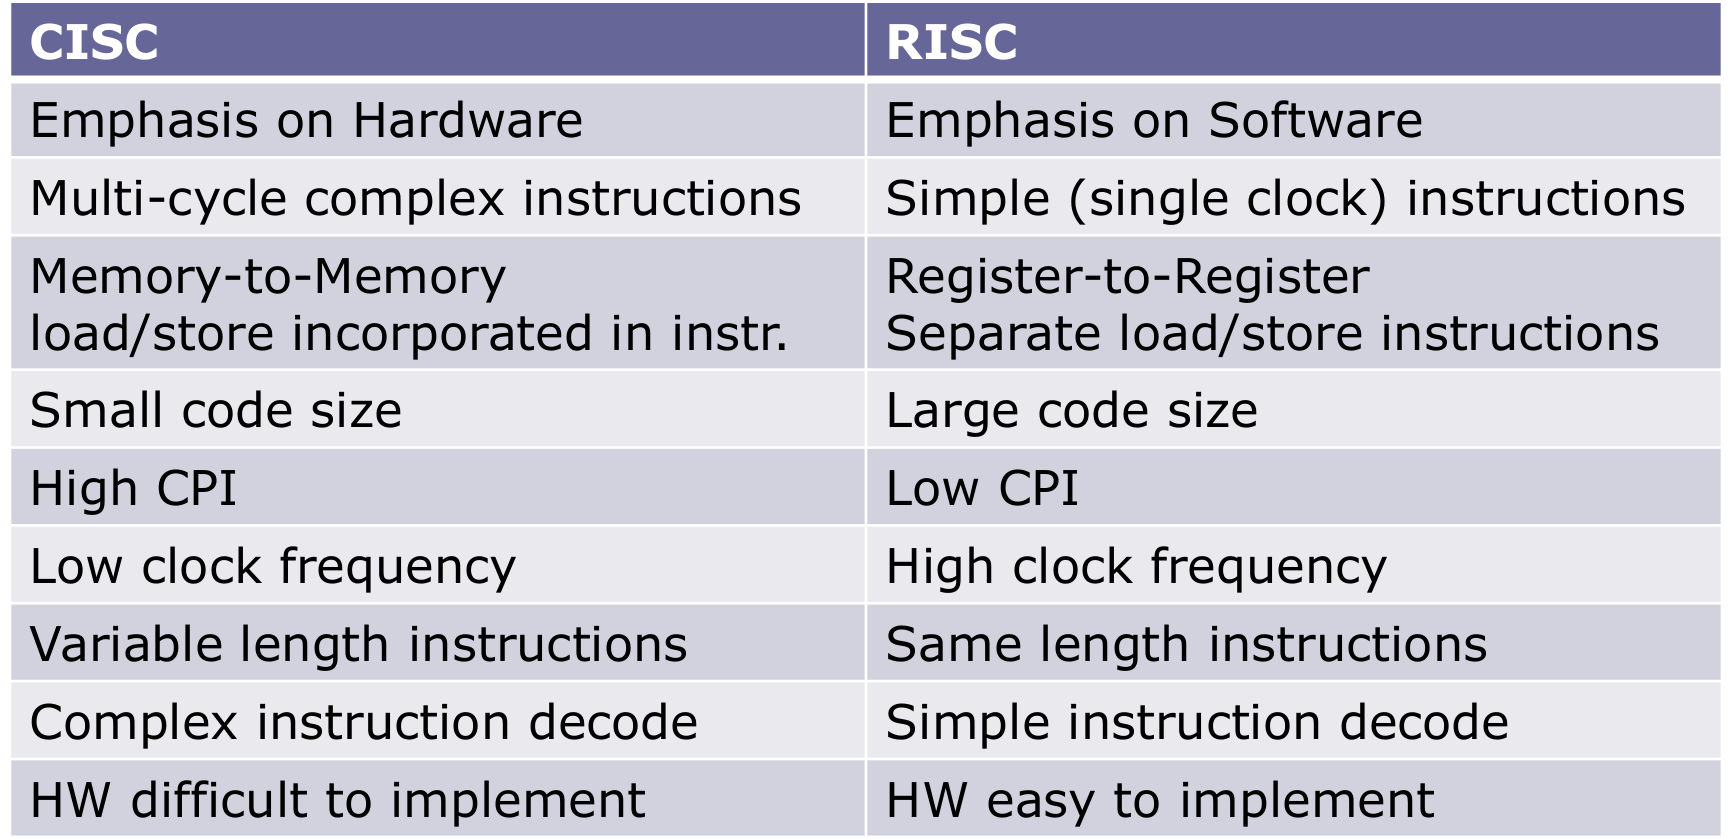
\includegraphics[width=\linewidth]{png/risc.png}
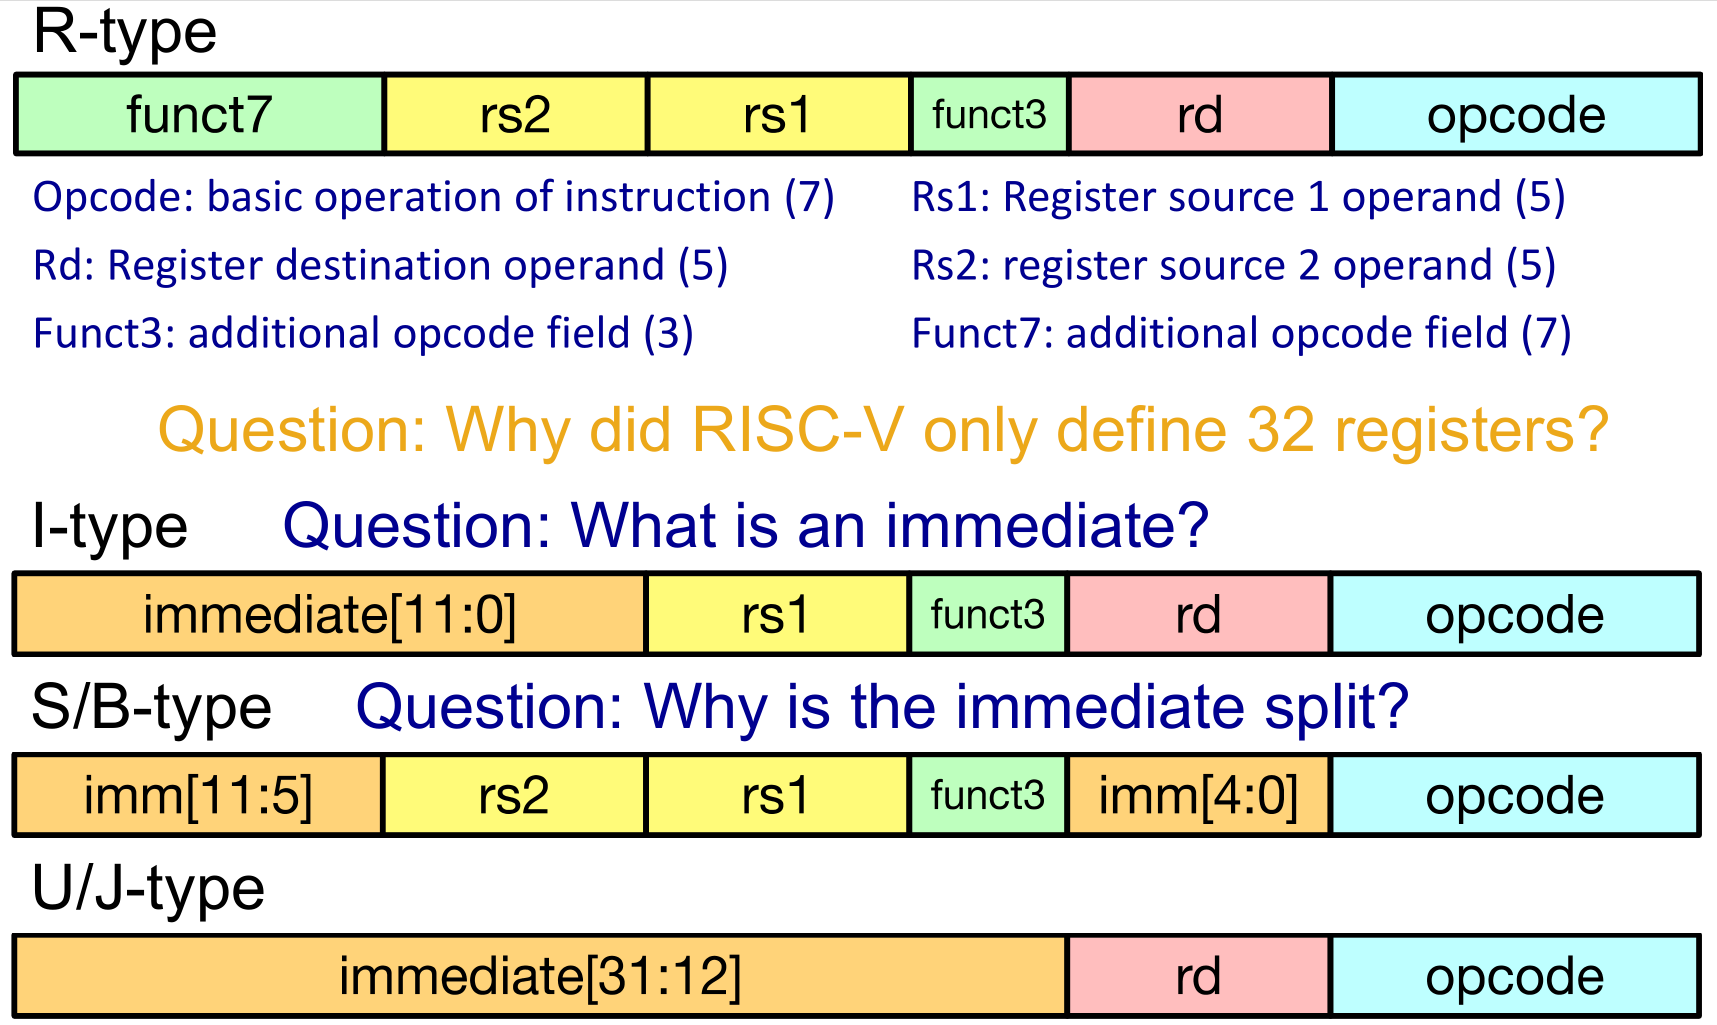
\includegraphics[width=\linewidth]{png/isa.png}
Constant == immediate == literal == offset

There are 32 registers in RISC-V
\textbf{ld dst, offset(base)} the base is the starting address of the array the
offset is the index

When using switch statement we can use a jump table, a jump table holds addresses
in memory of where the code for the jump targets are.

\textbf{Stack:} The stack is a allocated in frames, it stores the state of a
procedure for a limited time, the callee returns before the caller does. The
things which can be saved on the stack are: local arrays, return addresses,
saved registers, and nested call arguments

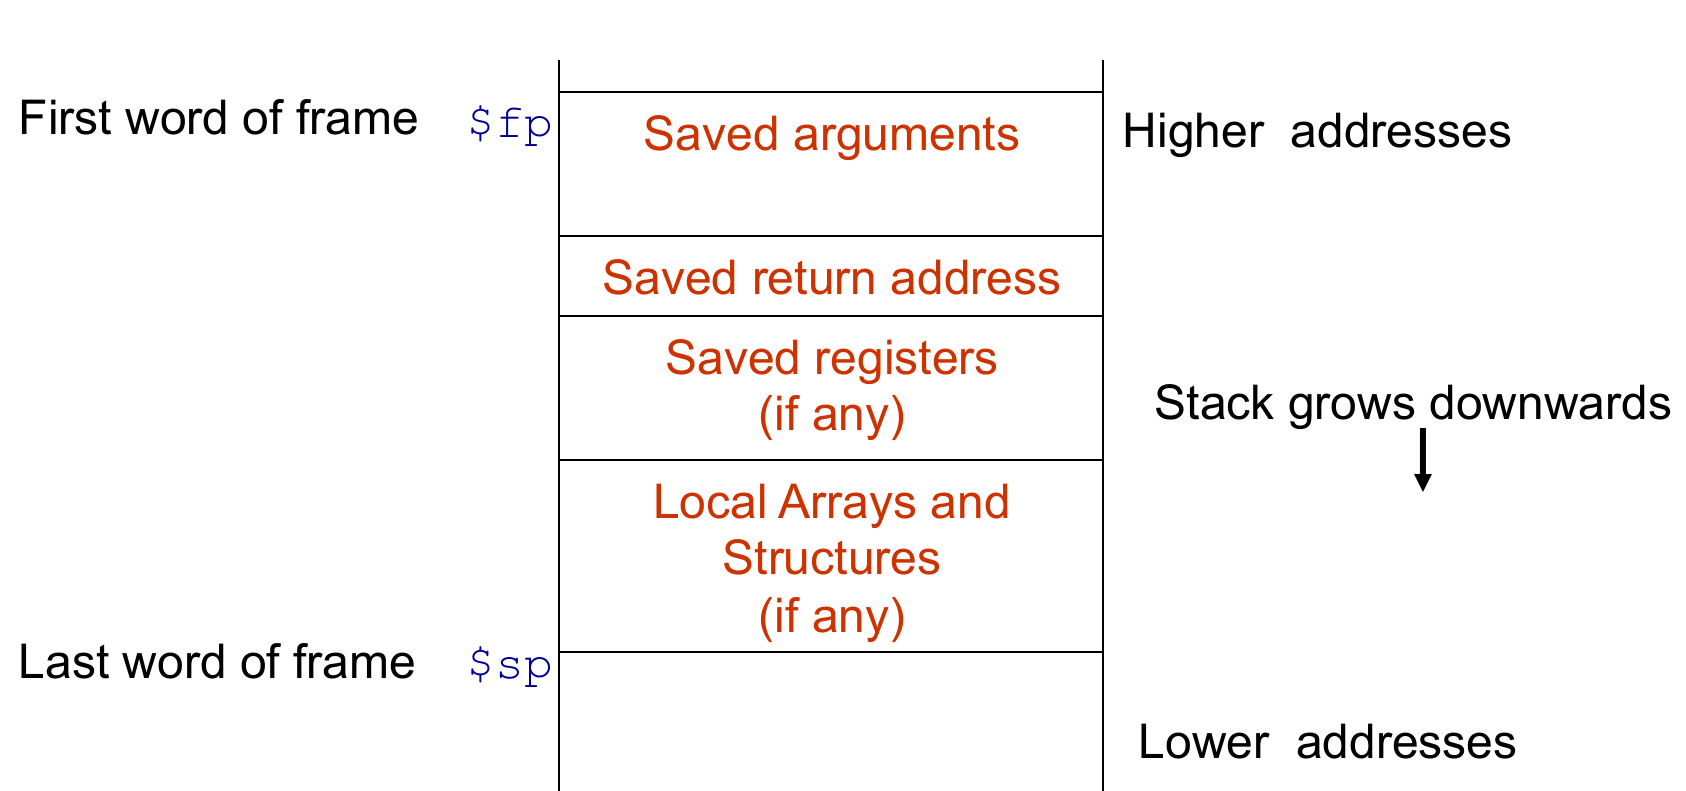
\includegraphics[width=\linewidth]{png/stack.png}
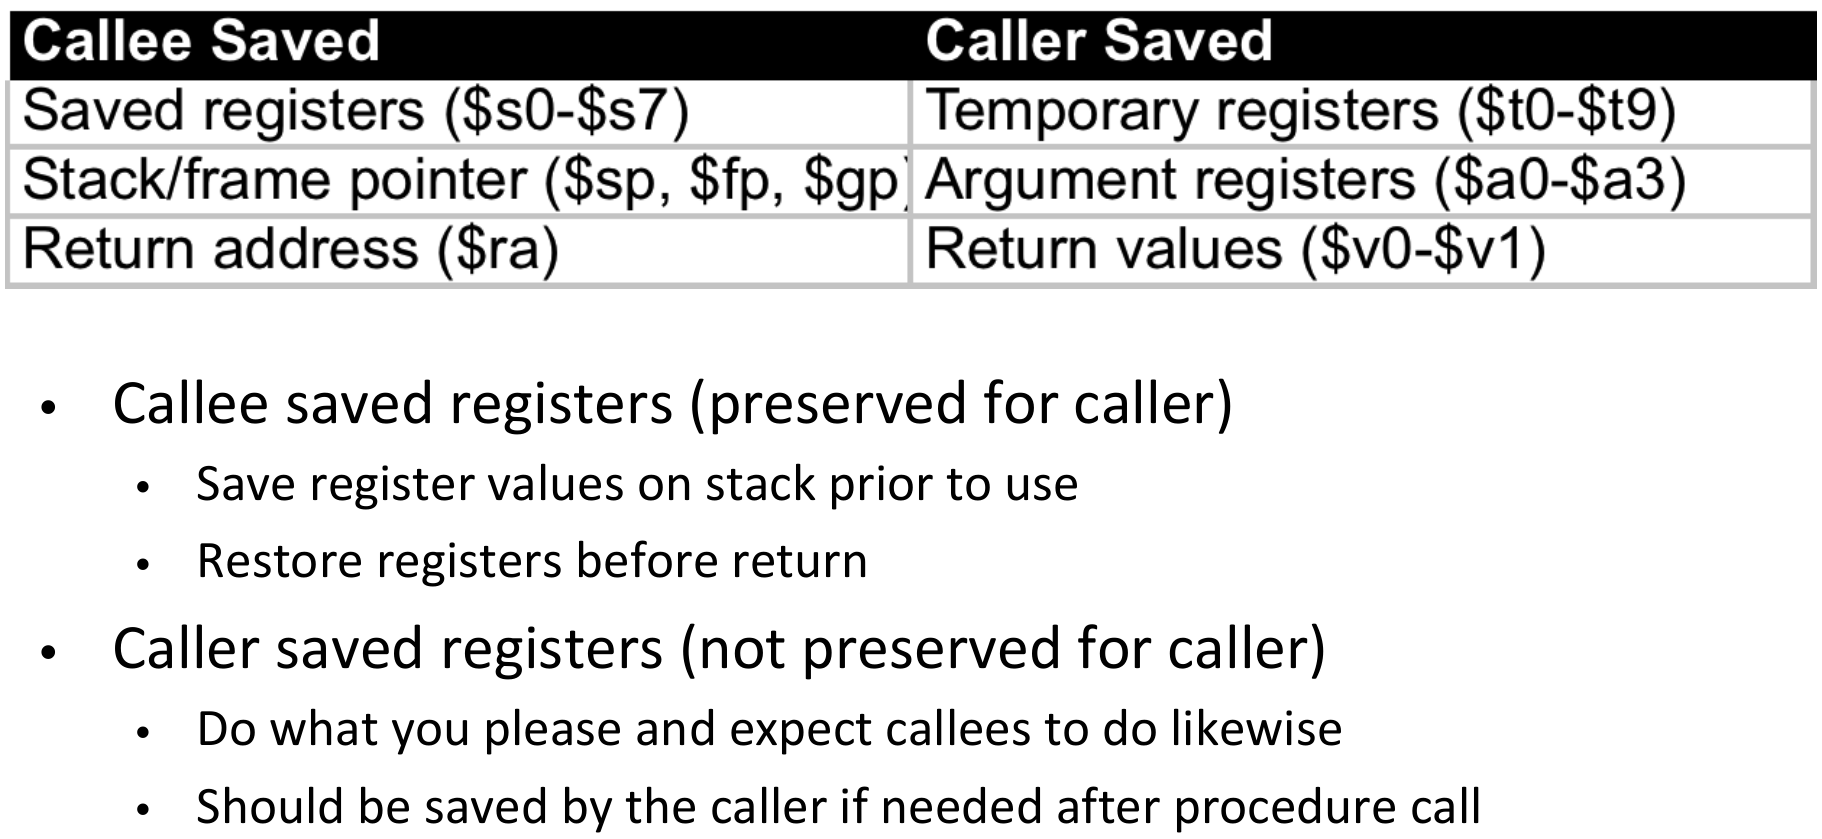
\includegraphics[width=\linewidth]{png/save.png}

\textbf{Procedure Call Steps}
\begin{enumerate}
\item Place parameters in a place where the procedure can access them
\item Transfer control to the procedure
\item Allocate the memory resources needed for the procedure
\item Perform the desired task
\item Place the result value in a place where the calling program can access it
\item Free the memory allocated in (3)
\item Return control to the point of origin
\end{enumerate}

\section{Pipelining}
In pipelinging we overlap instructions in defferent stages
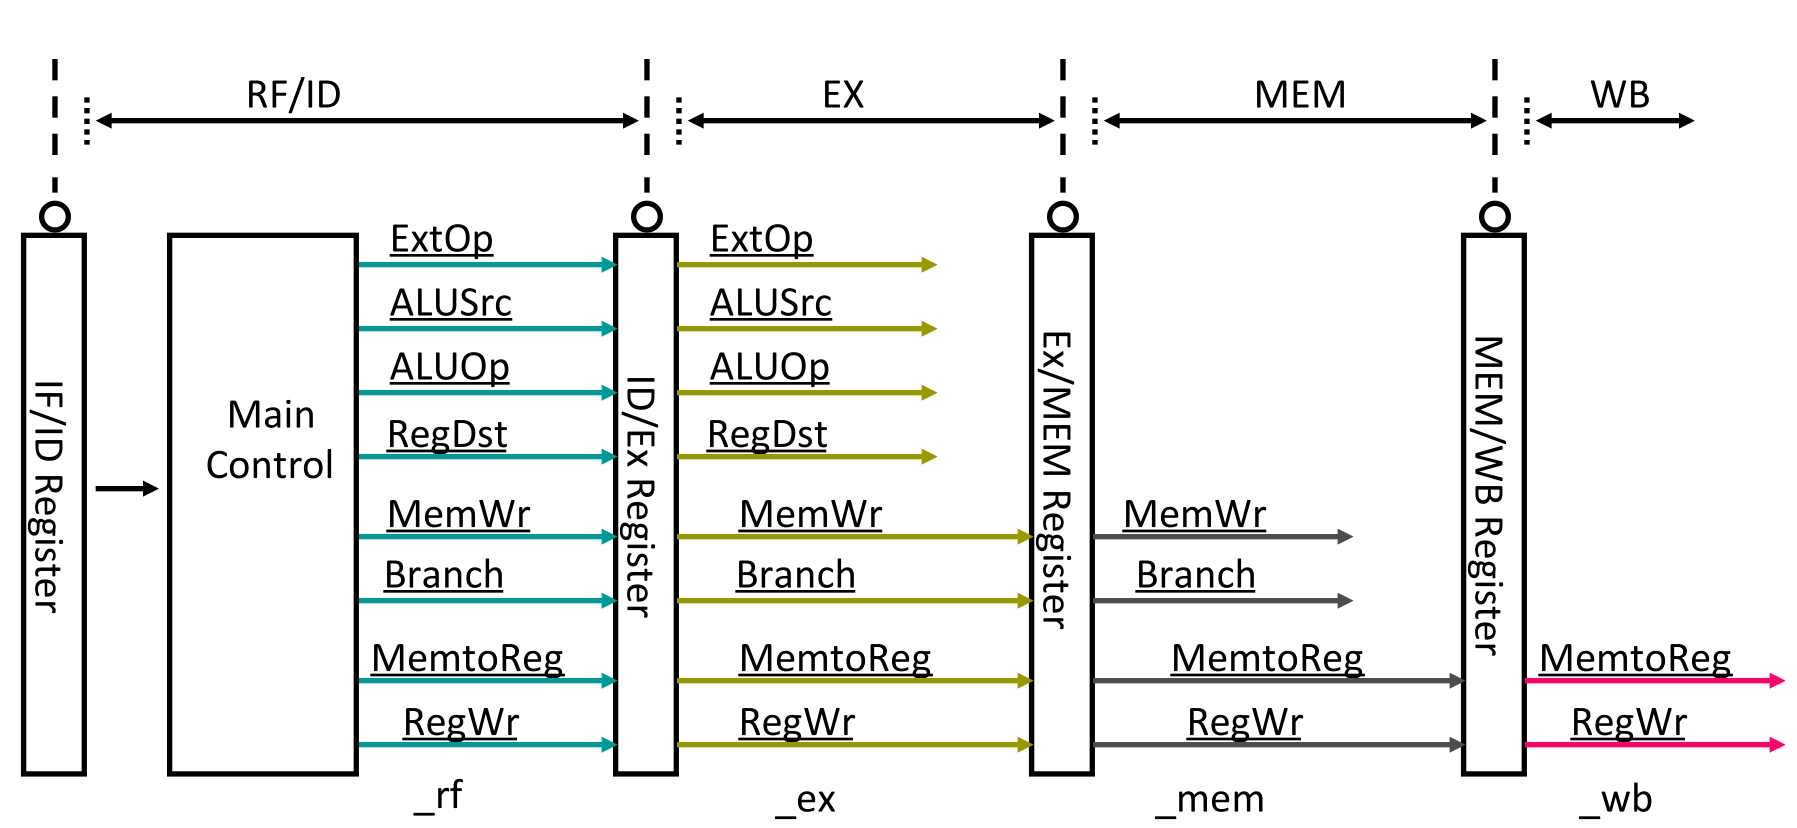
\includegraphics[width=\linewidth]{png/pipe.png}
There are hazards, these include \textbf{structural hazards}
where a required resource is busy, \textbf{data harzards} where we must wait previous
instructions to produce/consume data, and \textbf{control hazards} where next PC
depends on previous instruction.

\subsection*{Structural Hazards}
two instructions are trying to use the same hardware within the same cycle, to
solve this we can make all the instructions the same length

\subsection*{Data Dependencies}
Dependencies for instruction $j$ following instruction $i$
\begin{itemize}
\item Read after Write (RAW or true dependence)
	\par Instruction $j$ tries to read before instruction $i$ tries to write it
\item Write after Write (WAW or output dependence)
	\par Instruction $j$ tries to write an operand before $i$ writes its value
\item Write after Read (WAR or (anti dependence))
	\par Instruction $j$ tries to write a destination before it is read by $i$
\end{itemize}
\textbf{Solutions for RAW Hazards}: We can delay the reading of an instruction
until data is available, to do this we can insert pipeline bubbles, can also write
to the register file in the first half of a cycle and then read in the second half.

\textbf{Forwarding:} Another solution is forwarding or pushing the data to an
appropriate unit.

We can also reorder instructions to deal with RAW hazards
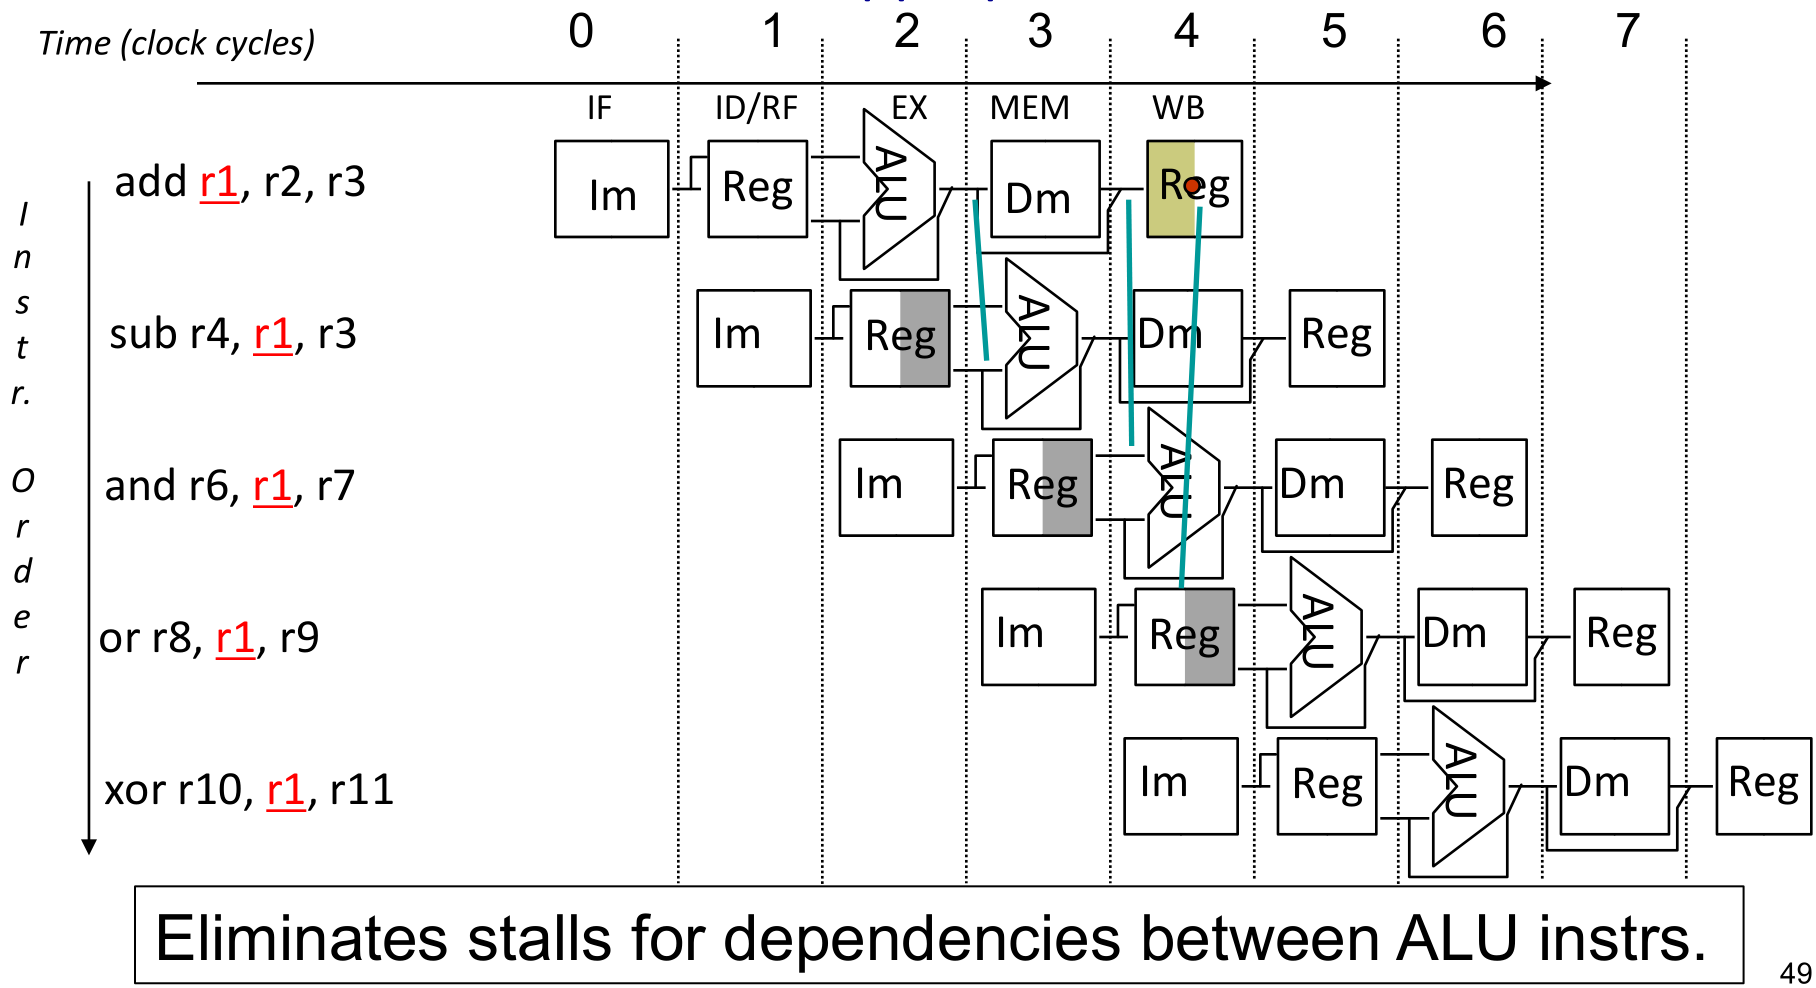
\includegraphics[width=\linewidth]{png/forwarding.png}
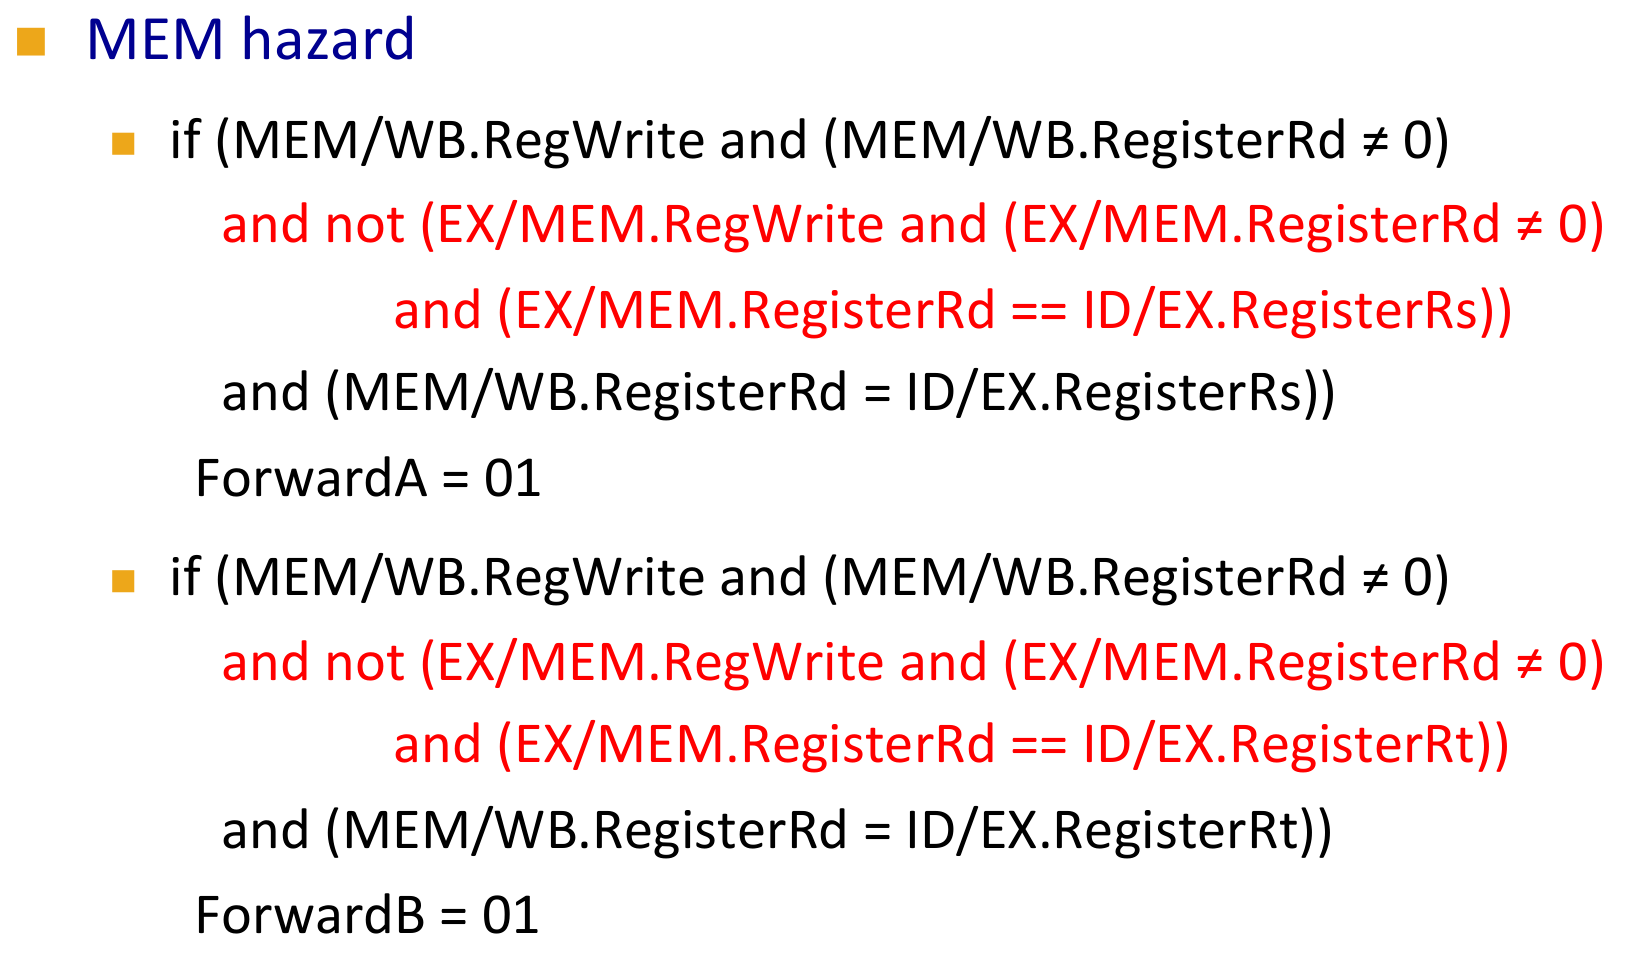
\includegraphics[width=\linewidth]{png/forwardingcontrol.png}

\subsection*{Control Hazards}
A control hazards is like a data hazard on the PC, we cannot fetch the next
instruction if we don't know the PC

Some solutions for control hazards are stalling on branches, predicting taken
or not taken. We need to flush the pipeline if we predict wrong, in a 5-sage
pipeline we only need to flush 1 instruction

\section{Out of Order Execution and ILP}
We want to avoid in-order stalls so we use out of order execution to re-order instructions based on dependencies\\
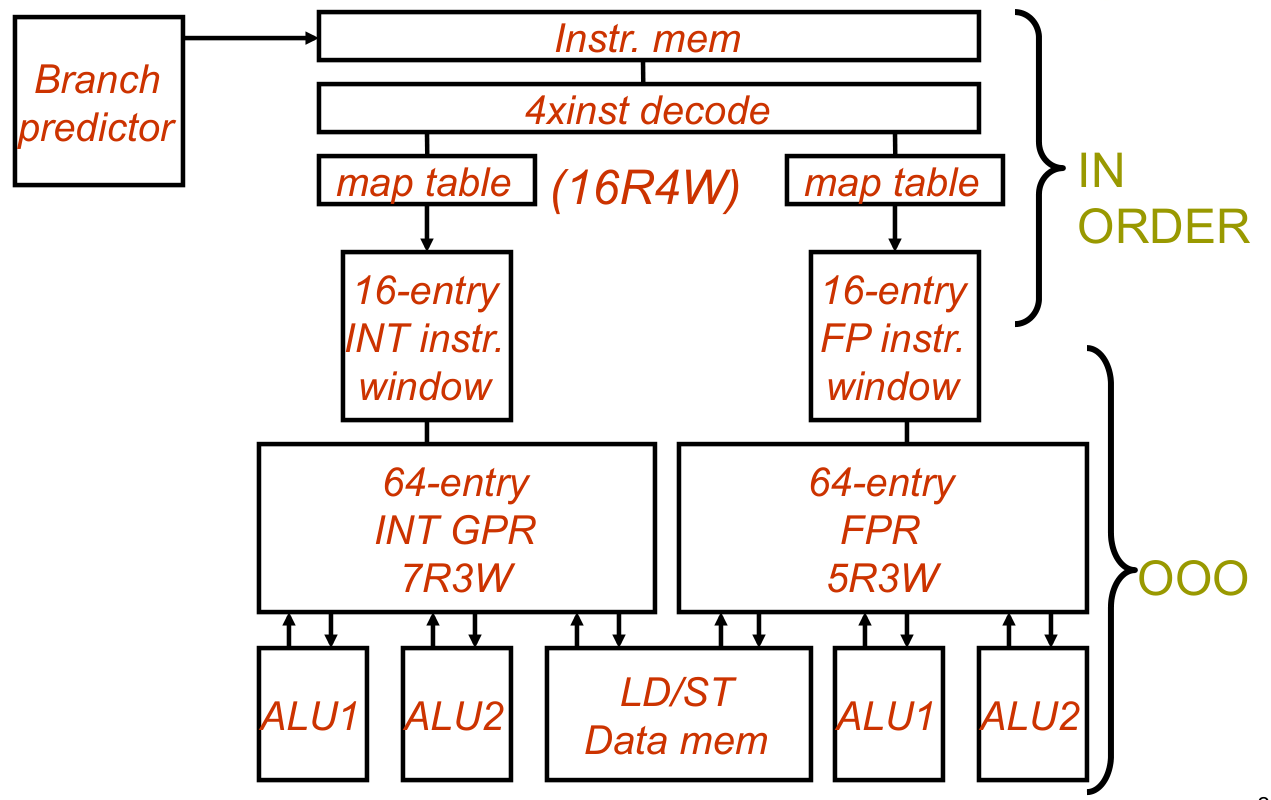
\includegraphics[width=\linewidth]{png/ooo.png}
A \textbf{superscalar processor} is a CPU that implements a form of parallelism
called instruction-level parallelism within a single processor. I.e we can launch
multiple instructions every cycle.\\

There are some issues with multiple instructions executing at onc,e we need to
double the amount of hardware, we introduce hazards, branch delay, \& load delay\\

We can rename (map) architectural registers to physical registers in decode stage
to get rid of false dependencies\\

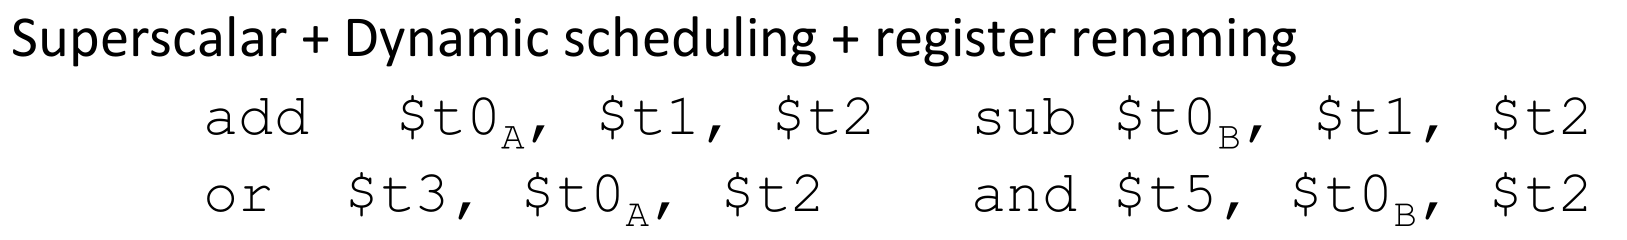
\includegraphics[width=\linewidth]{png/super.png}
There are some limits to \textbf{ILP} and pipelining:\\
Limited ILP in real programs\\
Pipeline overhead\\
Branch and load delays exacerbated\\
Clock cycle timing limits\\
Limited branch prediction accuracy (85\%-98\%)\\
Even a few percent really hurts with long/wide pipes!\\
Memory inefficiency\\
Load delays + \# of loads/cycle\\

\end{multicols*}
\end{document}
